\begin{frame}
    \frametitle{\problemtitle}
    \begin{block}{Problem}
        \begin{itemize}
            \item Given a convex polygon with internal angles $\geq 90^\circ$.
            \item Move one point to maximize the perimeter.
            \item The polygon must stay convex (angles $\leq 180^\circ$) and all internal angles $\geq 90^\circ$.
        \end{itemize}
    \end{block}

    \only<2->{
        \begin{block}{Solution}
            \begin{columns}
                \begin{column}{0.5\textwidth}
                        \begin{itemize}
                            \item<2-> Try to move every point individually.
                            \item<3-> The angle $\angle BCD$ is in $[90^\circ, 180^\circ]$ if $C$ stays within the Thales semicircle.
                            \item<4-> Ideally, we move $C$ to the middle top of the Thales semicircle.
                            \item<4-> This maximizes the perimeter.
                      \end{itemize}
                \end{column}
                \begin{column}{0.4\textwidth}
                    \only<2>{
                        \begin{figure}[thb]
                            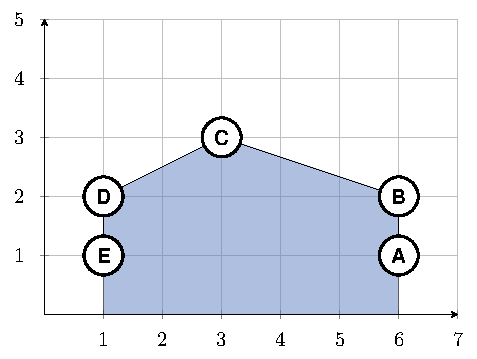
\includegraphics[scale=0.6]{solution-illustration1.pdf}
                        \end{figure}
                    }
                    \only<3>{
                        \begin{figure}[thb]
                            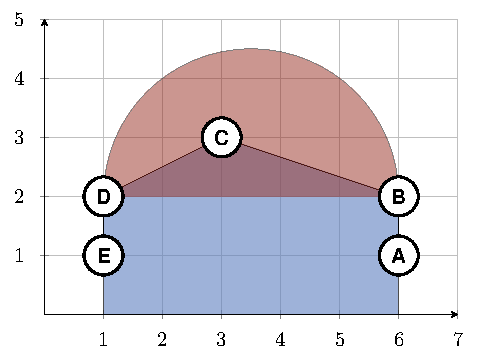
\includegraphics[scale=0.6]{solution-illustration8.pdf}
                        \end{figure}
                    }
                    \only<4>{
                        \begin{figure}[thb]
                            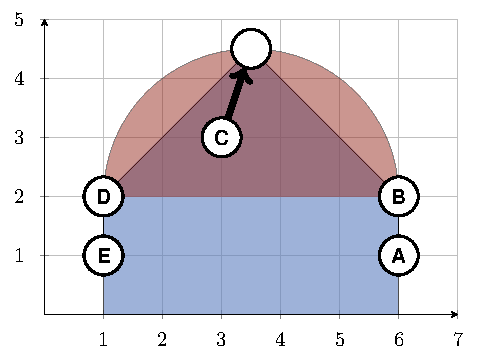
\includegraphics[scale=0.6]{solution-illustration2.pdf}
                        \end{figure}
                    }
                \end{column}
            \end{columns}
        \end{block}
    }
\end{frame}


\begin{frame}
    \begin{block}{Solution}
        \begin{itemize}
            \item<1-> Ideally, we move $C$ to the middle top of the Thales semicircle.
            \item<1-> This maximizes the perimeter.
            \item<1-> However, this is not always possible because of the angles $\angle ABC$ and $\angle CDE$.
      \end{itemize}
    \end{block}
    \only<1>{
        \begin{figure}[thb]
             \begin{minipage}{0.5\textwidth}
                \centering
                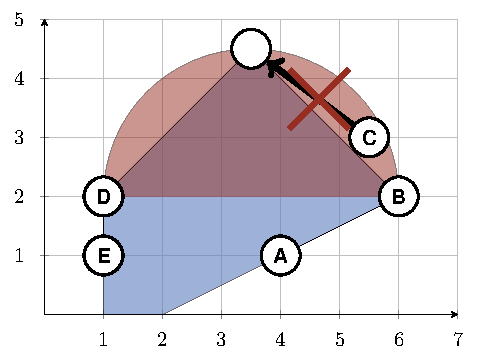
\includegraphics[scale=0.6]{solution-illustration4.pdf}
            \end{minipage}\hfill
            \begin{minipage}{0.5\textwidth}
                \centering
                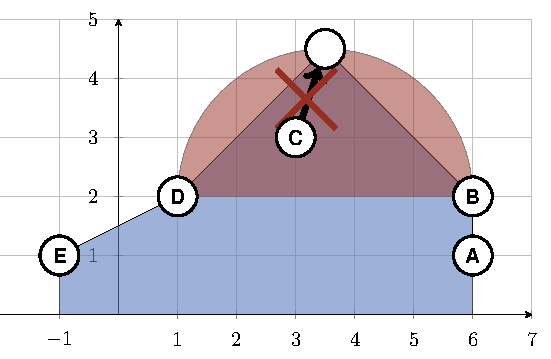
\includegraphics[scale=0.6]{solution-illustration3.pdf}
            \end{minipage}
        \end{figure}
    }
\end{frame}

\begin{frame}
    \begin{block}{Solution}
        \begin{itemize}
            \item<1-> The angle $\angle CDE$ is $\leq 180^\circ$, if $C$ stays in the green halfplane.
            \item<2-> By intuition or triangle inequality, the intersection point between halfplane line and Thales semicircle is optimal (or middle top of Thales circle).
            \item<3-> There is also a (pink) halfplane for $\angle CDE \geq 90^\circ$ (and $\leq 270^\circ$).
            \item<4-> One of the two halfplanes completely contains the semicircle, ignore that one.
      \end{itemize}
    \end{block}
    \only<1->{
        \begin{figure}[thb]
             \begin{minipage}{0.5\textwidth}
                \centering
                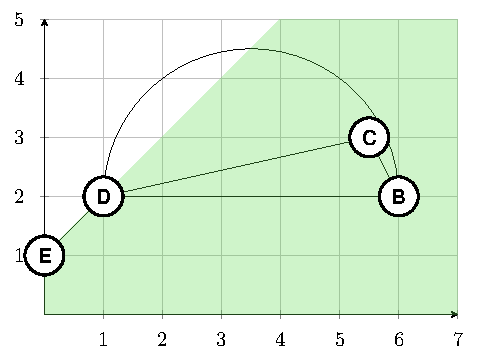
\includegraphics[scale=0.6]{solution-illustration5.pdf}
            \end{minipage}\hfill
            \begin{minipage}{0.5\textwidth}
                \only<3->{
                    \centering
                    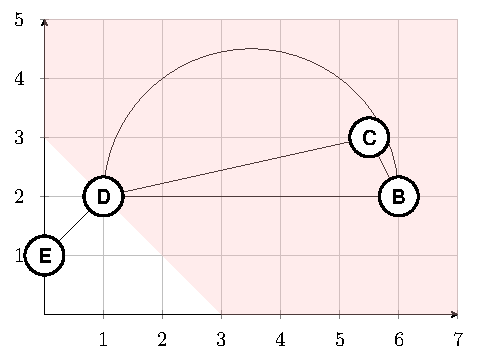
\includegraphics[scale=0.6]{solution-illustration6.pdf}
                }
            \end{minipage}
        \end{figure}
    }
\end{frame}

\begin{frame}
    \begin{block}{Solution}
        \begin{itemize}
            \item<1-> Both angles $\angle ABC$ and $\angle CDE$ have one relevant halfplane.
            \item<1-> The halfplane lines might intersect in the semicircle.
            \item<2-> Here, the intersection point of the lines is optimal.
      \end{itemize}
    \end{block}

    \bigskip
    \only<1->{
        \centering
        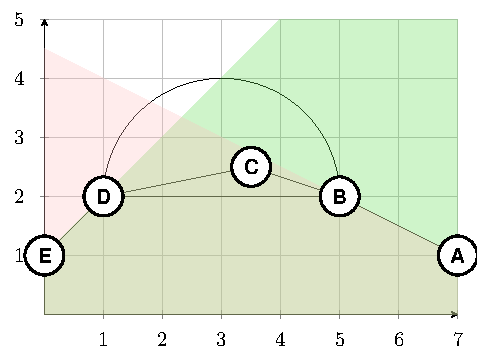
\includegraphics[scale=0.6]{solution-illustration7.pdf}
    }
\end{frame}

\begin{frame}
    \begin{block}{Solution}
        \begin{itemize}
            \item<1-> In total, there are four possible optimal points:
            \end{itemize}
        \begin{enumerate}
            \item<2-> Middle top of the Thales semicircle.
            \item<2-> Intersection $\angle ABC$ halfplane and Thales semicircle.
            \item<2-> Intersection $\angle CDE$ halfplane and Thales semicircle.
            \item<2-> Intersection $\angle ABC$ and $\angle CDE$ halfplane lines.
        \end{enumerate}
        \begin{itemize}
            \item<3-> Try all of these points and check whether they are valid.
            \item<4-> Take care of precision issues: Use \texttt{long double} and large $\varepsilon$ (e.g. $\varepsilon = 10^{-7}$).
            \item<4-> Runtime: $\mathcal{O}(n)$.
        \end{itemize}
    \end{block}
\end{frame}
